% 2025 全国 2 卷 17：正方形沿 EF 翻折后的四棱锥体（A、D 翻折到 A'、D'）
% 立体坐标 E(0,0,0)、B(2,0,0)、F(0,1,0)、C(1,1,0)、A'(1/2,0,√3/2)、D'(1/2,1,√3/2)，
% 翻折前的位置 A(-1,0,0)、D(-1,1,0) 以虚影正方形 AEFD 保留，示折痕 EF 的来源。
% 画布投影：(x,y,z) -> x·(1,0) + y·(0.35,0.45) + z·(0,1)。
% 虚线：被遮挡的 EF、FC、FD'、D'C，以及翻折前的虚影边 AE、AD、DF。
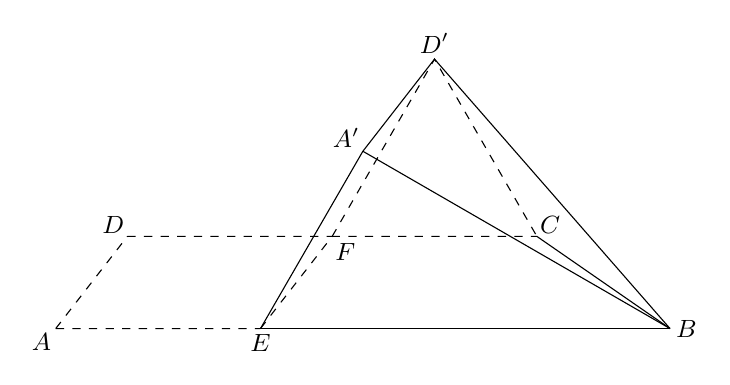
\begin{tikzpicture}[scale=2.6, font=\small]
  \coordinate (E)  at (0,0);
  \coordinate (B)  at (2,0);
  \coordinate (F)  at (0.35,0.45);
  \coordinate (C)  at (1.35,0.45);
  \coordinate (Ap) at (0.5,0.866);
  \coordinate (Dp) at (0.85,1.316);
  \coordinate (A)  at (-1,0);
  \coordinate (D)  at (-0.65,0.45);
  % 可见实线
  \draw (E) -- (B);
  \draw (E) -- (Ap) -- (Dp) -- (B);
  \draw (Ap) -- (B);
  \draw (C) -- (B);
  % 被遮挡
  \draw[dashed] (E) -- (F) -- (C);
  \draw[dashed] (F) -- (Dp) -- (C);
  % 翻折前的虚影正方形 AEFD
  \draw[dashed] (A) -- (E)  (A) -- (D)  (D) -- (F);
  \node[below left,  inner sep=1.5pt] at (A)  {$A$};
  \node[above left,  inner sep=1pt]   at (D)  {$D$};
  \node[below,       inner sep=2pt]   at (E)  {$E$};
  \node[below right, inner sep=1pt, yshift=-1.5pt] at (F) {$F$};
  \node[above right, inner sep=1pt]   at (C)  {$C$};
  \node[right,       inner sep=2pt]   at (B)  {$B$};
  \node[above left,  inner sep=1pt]   at (Ap) {$A'$};
  \node[above,       inner sep=2pt]   at (Dp) {$D'$};
\end{tikzpicture}
